\documentclass{beamer}
\usepackage{graphics}

% Beamer appearance
\usepackage{helvet}
\definecolor{MaltaBlue}{RGB}{81,118,147}
\definecolor{FireBrick}{RGB}{228,34,23}
\setbeamertemplate{navigation symbols}{}
\setbeamertemplate{headline}{} % removes navtree
\setbeamercolor{example text}{fg=black}
\setbeamercolor{footline}{fg=black}
\setbeamercolor{structure}{fg=black}
\setbeamercolor{alerted text}{fg=FireBrick}
\setbeamertemplate{footline}{\strut\hfill%
\insertframenumber~~}%/\inserttotalframenumber~~}

\title{Artisanal Type Theory}
\author{Carlo Angiuli}
\date{April 1, 2015}
\institute{Carnegie Mellon University}

\usebackgroundtemplate%
{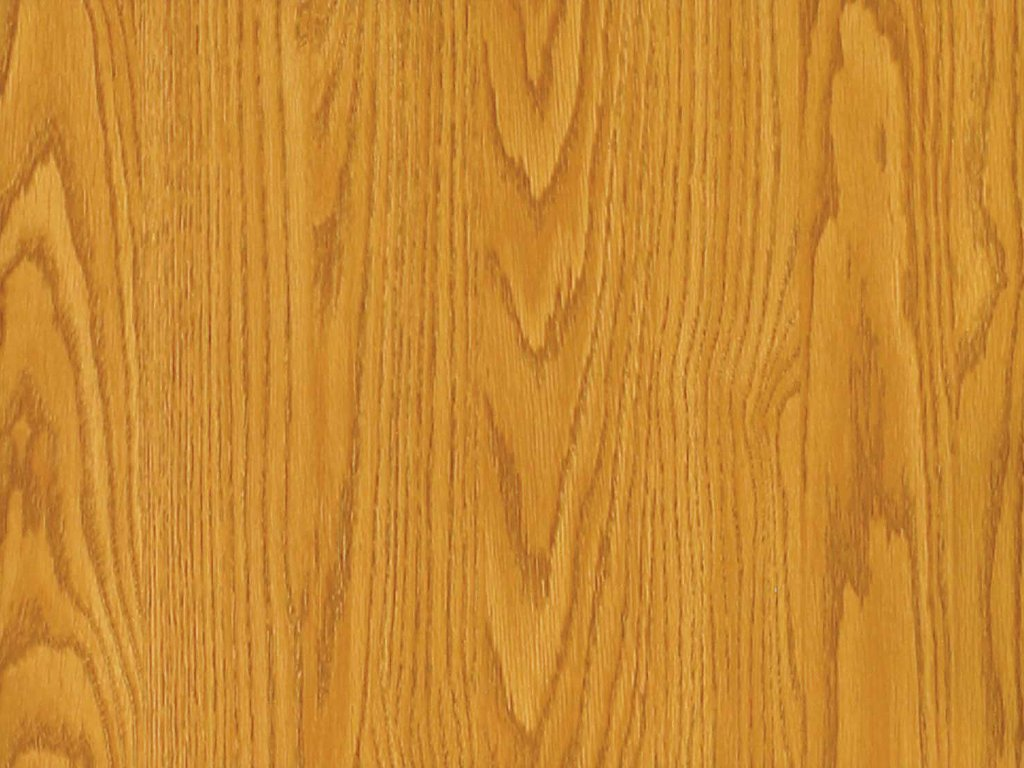
\includegraphics[width=\paperwidth,height=\paperheight]{bg.jpg}}

\begin{document}

\begin{frame}
\maketitle
\end{frame}

\begin{frame}
\begin{center}
Computers have ruined good, old-fashioned computing.
\end{center}
\end{frame}

\begin{frame}
\begin{center}
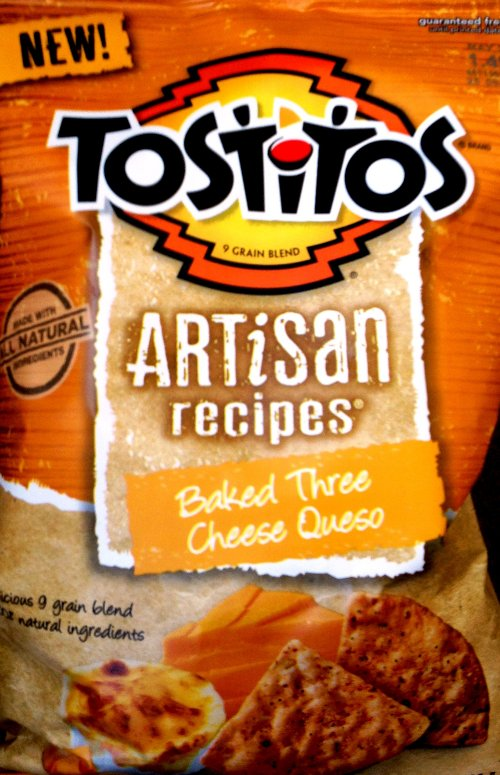
\includegraphics[width=2in]{tostitos.jpg}
\end{center}
\end{frame}

\begin{frame}
\begin{center}
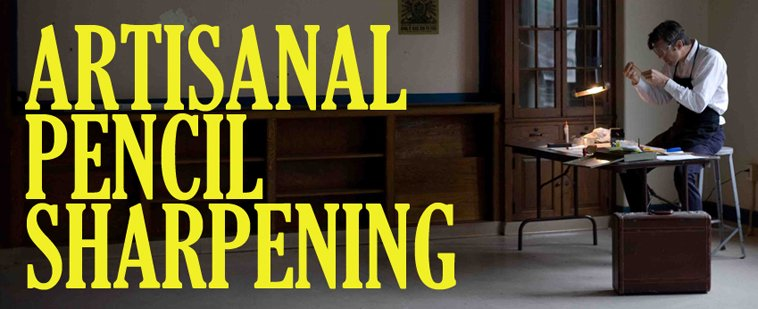
\includegraphics[width=4in]{pencil.jpg}
\end{center}
\end{frame}

\begin{frame}
\frametitle{Food with a human touch}
\end{frame}

\end{document}

